\bta{动能定理}


\begin{enumerate}[leftmargin=0em]
\renewcommand{\labelenumi}{\arabic{enumi}.}
% A(\Alph) a(\alph) I(\Roman) i(\roman) 1(\arabic)
%设定全局标号series=example	%引用全局变量resume=example
%[topsep=-0.3em,parsep=-0.3em,itemsep=-0.3em,partopsep=-0.3em]
%可使用leftmargin调整列表环境左边的空白长度 [leftmargin=0em]




\item
\exwhere{$ 2018 $年全国 \lmd{2} 卷}
如图,某同学用绳子拉动木箱,使它从静止开始沿粗糙水平路面运动至具有某一速度,木箱获得的动能一定 \xzanswer{A} 
\begin{figure}[h!]
\centering
\includesvg[width=0.23\linewidth]{picture/svg/750}
\end{figure}

\fourchoices
{小于拉力所做的功}
{等于拉力所做的功}
{等于克服摩擦力所做的功}
{大于克服摩擦力所做的功}


\item
\exwhere{$ 2016 $年新课标$ \lmd{3} $卷}
如图,一固定容器的内壁是半径为$ R $的半球面;在半球面水平直径的一端有一质量为$ m $的质点$ P $。它在容器内壁由静止下滑到最低点的过程中,克服摩擦力做的功为$ W $。重力加速度大小为$ g $。设质点$ P $在最低点时,向心加速度的大小为$ a $,容器对它的支持力大小为$ N $,则 \xzanswer{AC} 


\begin{minipage}[h!]{0.7\linewidth}
\vspace{0.3em}
\fourchoices
{$ a = \frac { 2 ( m g R - W ) } { m R } $}
{$ a = \frac { 2 m g R - W } { m R } $}
{$ N = \frac { 3 m g R - 2 W } { R } $}
{$ N = \frac { 2 ( m g R - W ) } { R } $}
\vspace{0.3em}
\end{minipage}
\hfill
\begin{minipage}[h!]{0.3\linewidth}
\flushright
\vspace{0.3em}
\includesvg[width=0.5\linewidth]{picture/svg/751}
\vspace{0.3em}
\end{minipage}



\item 
\exwhere{$ 2016 $年四川卷}
韩晓鹏是我国首位在冬奥会雪上项目夺冠的运动员。他在一次自由式滑雪空中技巧比赛中沿“助滑区”保持同一姿态下滑了一段距离,重力对他做功$ 1900 \ J $,他克服阻力做功$ 100 \ J $。韩晓鹏在此过程中 \xzanswer{C} 

\fourchoices
{动能增加了$ 1900 \ J $}
{动能增加了$ 2000 \ J $}
{重力势能减小了$ 1900 \ J $}
{重力势能减小了$ 2000 \ J $}



\item 
\exwhere{$ 2013 $年山东卷}
$ 16 $、如图所示,楔形木块$ abc $固定在水平面上,粗糙斜面$ ab $和光滑斜面$ bc $与水平面的夹角相同,顶角$ b $处安装一定滑轮,质量分别为$ M $、$ m $($ M>m $)的滑块,通过不可伸长的轻绳定滑轮连接,轻绳与斜面平行,两滑块由静止释放后,沿斜面做匀加速运动。若不计滑轮的质量和摩擦,在两滑块沿斜面运动的过程中 \xzanswer{CD} 


\begin{minipage}[h!]{0.7\linewidth}
\vspace{0.3em}
\fourchoices
{两滑块组成系统的机械能守恒}
{重力对$ M $做的功等于$ M $动能的增加}
{轻绳对$ m $做的功等于$ m $机械能的增加}
{两滑块组成系统的机械能损失等于$ M $克服摩擦力做的功}

\vspace{0.3em}
\end{minipage}
\hfill
\begin{minipage}[h!]{0.3\linewidth}
\flushright
\vspace{0.3em}
\includesvg[width=0.9\linewidth]{picture/svg/752}
\vspace{0.3em}
\end{minipage}



\item
\exwhere{$ 2011 $年新课标卷}
一质点开始时做匀速直线运动,从某时刻起受到一恒力作用。此后,该质点的动能可能 \xzanswer{ABD} 

\fourchoices
{一直增大}
{先逐渐减小至零,再逐渐增大}
{先逐渐增大至某一最大值,再逐渐减小}
{先逐渐减小至某一非零的最小值,再逐渐增大}




\item 
\exwhere{$ 2014 $年理综大纲卷}
一物块沿倾角为$ \theta $的斜坡向上滑动。当物块的初速度为$ v $时,上升的最大高度为$ H $,如图所示;当物块的初速度为$ \frac{v}{2} $时,上升的最大高度记为$ h $。重力加速度大小为$ g $。物块与斜坡间的动摩擦因数和$ h $分别为 \xzanswer{D} 
\begin{figure}[h!]
\centering
\includesvg[width=0.23\linewidth]{picture/svg/753}
\end{figure}

\fourchoices
{$ \tan \theta \text{和} \frac { H } { 2 } $}
{$ \left( \frac { v ^ { 2 } } { 2 g H } - 1 \right) \tan \theta \text{和} \frac { H } { 2 } $}
{$ \tan \theta \text{和} \frac { H } { 4 } $}
{$ \left( \frac { v ^ { 2 } } { 2 g H } - 1 \right) \tan \theta \text{和} \frac { H } { 4 } $}



\item 
\exwhere{$ 2017 $年江苏卷}
一小物块沿斜面向上滑动,然后滑回到原处。物块初动能为$ E_{k0} $,与斜面间的动摩擦因数不变,则该过程中,物块的动能$ E_{k} $与位移$ x $关系的图线是 \xzanswer{C} 
\begin{figure}[h!]
\centering
\includesvg[width=0.83\linewidth]{picture/svg/754}
\end{figure}

\item 
\exwhere{$ 2011 $年理综山东卷}
如图所示,将小球$ a $从地面以初速度$ v_{0} $竖直上抛的同时,将另一相同质量的小球$ b $从距地面$ h $处由静止释放,两球恰在$ h/2 $处相遇(不计空气阻力)。则 \xzanswer{C} 
\begin{figure}[h!]
\centering
\includesvg[width=0.1\linewidth]{picture/svg/755}
\end{figure}

\fourchoices
{两球同时落地}
{相遇时两球速度大小相等}
{从开始运动到相遇,球$ a $动能的减少量等于球$ b $动能的增加量}
{相遇后的任意时刻,重力对球$ a $做功功率和对球$ b $做功功率相等}



\item
\exwhere{$ 2015 $年海南卷}
如图,一半径为$ R $的半圆形轨道竖直固定放置,轨道两端等高;质量为$ m $的质点自轨道端点$ P $由静止开始滑下,滑到最低点$ Q $时,对轨道的正压力为$ 2mg $,重力加速度大小为$ g $,质点自$ P $滑到$ Q $的过程中,克服摩擦力所做的功为 \xzanswer{C} 
\begin{figure}[h!]
\centering
\includesvg[width=0.23\linewidth]{picture/svg/756}
\end{figure}

\fourchoices
{$ \frac { 1 } { 4 } m g R $}
{$ \frac { 1 } { 3 } m g R $}
{$ \frac { 1 } { 2 } m g R $}
{$ \frac { \pi } { 4 } m g R $}



\item 
\exwhere{$ 2016 $年浙江卷}
如图所示为一滑草场。某条滑道由上下两段高均为$ h $,与水平面倾角分别为$ 45 ^{ \circ } $和$ 37 ^{ \circ } $的滑道组成,滑草车与草地之间的动摩擦因数为$ \mu $。质量为$ m $的载人滑草车从坡顶由静止开始自由下滑,经过上、下两段滑道后,最后恰好静止于滑道的底端(不计滑草车在两段滑道交接处的能量损失,)。则 \xzanswer{AB} 
\begin{figure}[h!]
\centering
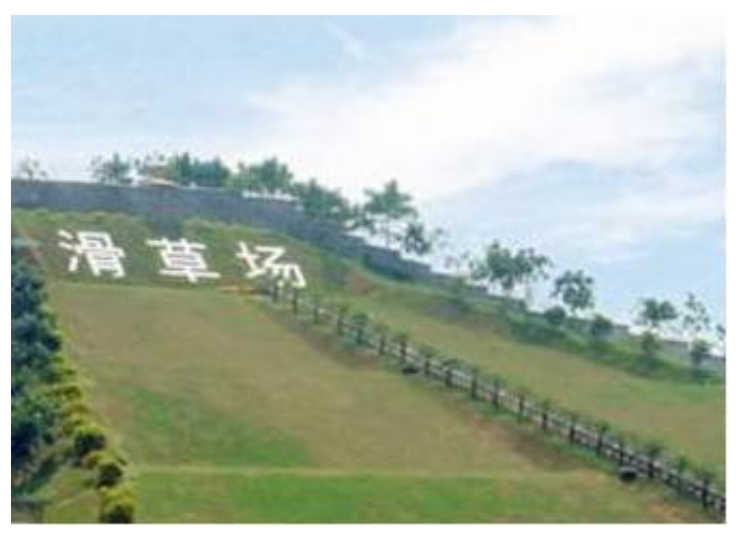
\includegraphics[width=0.23\linewidth]{picture/screenshot016}
\end{figure}

\fourchoices
{动摩擦因数$ \mu= \frac{ 6 }{ 7 } $}
{载人滑草车最大速度为$\sqrt { \frac { 2 g h } { 7 } }$}
{载人滑草车克服摩擦力做功为$ mgh $}
{载人滑草车在下段滑道上的加速度大小为$\frac { 3 } { 5 } g$}




\item 
\exwhere{$ 2016 $年天津卷}
我国高铁技术处于世界领先水平,和谐号动车组是由动车和拖车编组而成,提供动力的车厢叫动车,不提供动力的车厢叫拖车。假设动车组各车厢质量均相等,动车的额定功率都相同,动车组在水平直轨道上运行过程中阻力与车重成正比,某列动车组由$ 8 $节车厢组成,其中第$ 1 $、$ 5 $节车厢为动车,其余为拖车,则该动车组 \xzanswer{BD} 


\fourchoices
{启动时乘客受到车厢作用力的方向与车运动的方向相反}
{做匀加速运动时,第$ 5 $、$ 6 $节与第$ 6 $、$ 7 $节车厢间的作用力之比为$ 3:2 $}
{进站时从关闭发动机到停下来滑行的距离与关闭发动机时的速度成正比}
{与改为$ 4 $节动车带$ 4 $节拖车的动车组最大速度之比为$ 1:2 $}





\item 
\exwhere{$ 2011 $年上海卷}
以初速为$ v_{0} $,射程为$ s $的平抛运动轨迹制成一光滑轨道。一物体由静止开始从轨道顶端滑下,当其到达轨道底部时,物体的速率为 \tk{$\frac { g S } { v _ { 0 } }$} 
,其水平方向的速度大小为 \tk{$\frac { v _ { 0 } } { \sqrt { 1 + \left( v _ { 0 } ^ { 2 } / g S \right) ^ { 2 } } }$}。



\newpage
\item
\exwhere{$ 2016 $年上海卷}
风洞是研究空气动力学的实验设备。如图,将刚性杆水平固定在风洞内距地面高度$ H=3.2m $处,杆上套一质量$ m=3 \ kg $,可沿杆滑动的小球。将小球所受的风力调节为$ F=15 \ N $,方向水平向左。小球以初速度$ v_{0} =8 \ m/s $向右离开杆端,假设小球所受风力不变,取$ g=10 \ m/s^{2} $。求:
\begin{enumerate}
\renewcommand{\labelenumi}{\arabic{enumi}.}
% A(\Alph) a(\alph) I(\Roman) i(\roman) 1(\arabic)
%设定全局标号series=example	%引用全局变量resume=example
%[topsep=-0.3em,parsep=-0.3em,itemsep=-0.3em,partopsep=-0.3em]
%可使用leftmargin调整列表环境左边的空白长度 [leftmargin=0em]
\item
小球落地所需时间和离开杆端的水平距离;
\item 
小球落地时的动能。
\item 
小球离开杆端后经过多少时间动能为$ 78 \ J $?




\end{enumerate}
\begin{figure}[h!]
\flushright
\includesvg[width=0.25\linewidth]{picture/svg/757}
\end{figure}


\banswer{
\begin{enumerate}
\renewcommand{\labelenumi}{\arabic{enumi}.}
% A(\Alph) a(\alph) I(\Roman) i(\roman) 1(\arabic)
%设定全局标号series=example	%引用全局变量resume=example
%[topsep=-0.3em,parsep=-0.3em,itemsep=-0.3em,partopsep=-0.3em]
%可使用leftmargin调整列表环境左边的空白长度 [leftmargin=0em]
\item
$ 4.8\ m $
\item 
$ 120 \ J $
\item 
$ 0.24\ s $ 或$ 0.4\ s $

\end{enumerate}


}



\item
\exwhere{$ 2017 $年江苏卷}
如图所示,两个半圆柱$ A $、$ B $紧靠着静置于水平地面上,其上有一光滑圆柱$ C $,三者半径均为$ R $,$ C $的质量为$ m $,$ A $、$ B $的质量都为$ \frac{m}{2} $,与地面的动摩擦因数均为$ \mu $.现用水平向右的力拉$ A $,使$ A $缓慢移动,直至$ C $恰好降到地面.整个过程中$ B $保持静止.设最大静摩擦力等于滑动摩擦力,重力加速度为$ g $.求:
\begin{enumerate}
\renewcommand{\labelenumi}{\arabic{enumi}.}
% A(\Alph) a(\alph) I(\Roman) i(\roman) 1(\arabic)
%设定全局标号series=example	%引用全局变量resume=example
%[topsep=-0.3em,parsep=-0.3em,itemsep=-0.3em,partopsep=-0.3em]
%可使用leftmargin调整列表环境左边的空白长度 [leftmargin=0em]
\item
未拉$ A $时,$ C $受到$ B $作用力的大小$ F $;
\item 
动摩擦因数的最小值$ \mu _{min} $;
\item 
$ A $移动的整个过程中,拉力做的功$ W $.



\end{enumerate}
\begin{figure}[h!]
\flushright
\includesvg[width=0.25\linewidth]{picture/svg/758}
\end{figure}

\banswer{
\begin{enumerate}
\renewcommand{\labelenumi}{\arabic{enumi}.}
% A(\Alph) a(\alph) I(\Roman) i(\roman) 1(\arabic)
%设定全局标号series=example	%引用全局变量resume=example
%[topsep=-0.3em,parsep=-0.3em,itemsep=-0.3em,partopsep=-0.3em]
%可使用leftmargin调整列表环境左边的空白长度 [leftmargin=0em]
\item
$F = \frac { \sqrt { 3 } } { 3 } m g$
\item 
$u _ { \min } = \frac { \sqrt { 3 } } { 2 }$
\item 
$W = ( 2 \mu - 1 ) ( \sqrt { 3 } - 1 ) m g R$



\end{enumerate}


}


\newpage
\item 
\exwhere{$ 2012 $年理综北京卷}
如图所示,质量为$ m $的小物块在粗糙水平桌面上做直线运动,经距离$ l $后以速度$ v $飞离桌面,最终落在水平地面上。已知$ l=1.4\ m $,$ v=3.0 \ m/s $,$ m=0.10 \ kg $,物块与桌面间的动摩擦因数$ \mu =0.25 $,桌面高$ h=0.45\ m $.。不计空气阻力,重力加速度$ g $取$ 10 \ m/s^{2} $。求:
\begin{enumerate}
\renewcommand{\labelenumii}{(\arabic{enumii})}
\item 
小物块落地点距飞出点的水平距离$ s $;


\item 
小物块落地时的动能$ E_{k} $;


\item 
小物块的初速度大小$ v_{0} $。

\end{enumerate}
\begin{figure}[h!]
\flushright
\includesvg[width=0.25\linewidth]{picture/svg/759}
\end{figure}


\banswer{
\begin{enumerate}
\renewcommand{\labelenumi}{\arabic{enumi}.}
% A(\Alph) a(\alph) I(\Roman) i(\roman) 1(\arabic)
%设定全局标号series=example	%引用全局变量resume=example
%[topsep=-0.3em,parsep=-0.3em,itemsep=-0.3em,partopsep=-0.3em]
%可使用leftmargin调整列表环境左边的空白长度 [leftmargin=0em]
\item
$ s=0.9\ m $
\item 
$ E_{k}=0.90\ J $
\item 
$ v_{0}=4.0\ m/s $

\end{enumerate}


}




\item
\exwhere{$ 2012 $年物理江苏卷}
某缓冲装置的理想模型如图所示,劲度系数足够大的轻质弹簧与轻杆相连,轻杆可在固定的槽内移动,与槽间的滑动摩擦力恒为$ f $. 轻杆向右移动不超过$ l $ 时,装置可安全工作。 一质量为$ m $的小车若以速度$ v_{0} $ 撞击弹簧,将导致轻杆向右移动$ \frac{l}{4} $. 轻杆与槽间的最大静摩擦力等于滑动摩擦力,且不计小车与地面的摩擦。. 
\begin{enumerate}
\renewcommand{\labelenumii}{(\arabic{enumii})}
\item 
若弹簧的劲度系数为$ k $,求轻杆开始移动时,弹簧的压缩量$ x $; 


\item 
求为使装置安全工作,允许该小车撞击的最大速度$ v_m $; 


\item 
讨论在装置安全工作时,该小车弹回速度$ v ^{\prime} $和撞击速度$ v $的关系. 



\end{enumerate}
\begin{figure}[h!]
\flushright
\includesvg[width=0.34\linewidth]{picture/svg/760}
\end{figure}

\banswer{
\begin{enumerate}
\renewcommand{\labelenumi}{\arabic{enumi}.}
% A(\Alph) a(\alph) I(\Roman) i(\roman) 1(\arabic)
%设定全局标号series=example	%引用全局变量resume=example
%[topsep=-0.3em,parsep=-0.3em,itemsep=-0.3em,partopsep=-0.3em]
%可使用leftmargin调整列表环境左边的空白长度 [leftmargin=0em]
\item
$x = \frac { f } { k }$
\item 
$v _ { m } = \sqrt { v _ { 0 } ^ { 2 } + \frac { 3 f l } { 2 m } }$
\item 
当$v < \sqrt { v _ { 0 } ^ { 2 } - \frac { f l } { 2 m } }$时,$v ^ { \prime } = v$ \\
当$\sqrt { v _ { 0 } ^ { 2 } - \frac { f l } { 2 m } } \leq v \leq \sqrt { v _ { 0 } ^ { 2 } + \frac { 3 f l } { 2 m } }$时,$v ^ { \prime } = \sqrt { v _ { 0 } ^ { 2 } - \frac { f l } { 2 m } }$

\end{enumerate}


}




\newpage
\item
\exwhere{$ 2012 $年理综福建卷}
如图,用跨过光滑定滑轮的缆绳将海面上一艘失去动力的小船沿直线拖向岸边。已知拖动缆绳的电动机功率恒为$ P $,小船的质量为$ m $,小船受到的阻力大小恒为$ f $,经过$ A $点时的速度大小为$ v_{0} $,小船从$ A $点沿直线加速运动到$ B $点经历时间为$ t_{1} $,$ A $、$ B $两点间距离为$ d $,缆绳质量忽略不计。求:
\begin{enumerate}
\renewcommand{\labelenumi}{\arabic{enumi}.}
% A(\Alph) a(\alph) I(\Roman) i(\roman) 1(\arabic)
%设定全局标号series=example	%引用全局变量resume=example
%[topsep=-0.3em,parsep=-0.3em,itemsep=-0.3em,partopsep=-0.3em]
%可使用leftmargin调整列表环境左边的空白长度 [leftmargin=0em]
\item
小船从$ A $点运动到$ B $点的全过程克服阻力做的功$ W_{1} $;
\item 
小船经过$ B $点时的速度大小$ v_{1} $;
\item 
小船经过$ B $点时的加速度大小$ a $。



\end{enumerate}
\begin{figure}[h!]
\flushright
\includesvg[width=0.33\linewidth]{picture/svg/761}
\end{figure}


\banswer{
\begin{enumerate}
\renewcommand{\labelenumi}{\arabic{enumi}.}
% A(\Alph) a(\alph) I(\Roman) i(\roman) 1(\arabic)
%设定全局标号series=example	%引用全局变量resume=example
%[topsep=-0.3em,parsep=-0.3em,itemsep=-0.3em,partopsep=-0.3em]
%可使用leftmargin调整列表环境左边的空白长度 [leftmargin=0em]
\item
$W = F S = f d$
\item 
$v _ { 1 } = \sqrt { \frac { 2 ( P t - f d ) } { m } + v _ { 0 } ^ { 2 } }$
\item 
$a = \frac { P } { \sqrt { m ^ { 2 } v ^ { 2 } + 2 m ( P t - f d ) } } - \frac { f } { m }$



\end{enumerate}


}





\item 
\exwhere{$ 2015 $年理综浙江卷}
如图所示,用一块长$ L_{1} =1.0 \ m $的木板在墙和桌面间架设斜面,桌面高$ H=0.8 \ m $,长$ L_{2} =1.5 \ m $。斜面与水平桌面的倾角$ \theta $可在$ 0 \sim 60 ^{ \circ } $间调节后固定。将质量$ m=0.2 \ kg $的小物块从斜面顶端静止释放,物块与斜面间的动摩擦因数$ \mu _{1}=0.05 $,物块与桌面间的动摩擦因数$ \mu _{2} $,忽略物块在斜面与桌面交接处的能量损失。(重力加速度$ g $取$ 10 \ m/s^{2} $;最大静摩擦力等于滑动摩擦力)
\begin{enumerate}
\renewcommand{\labelenumi}{\arabic{enumi}.}
% A(\Alph) a(\alph) I(\Roman) i(\roman) 1(\arabic)
%设定全局标号series=example	%引用全局变量resume=example
%[topsep=-0.3em,parsep=-0.3em,itemsep=-0.3em,partopsep=-0.3em]
%可使用leftmargin调整列表环境左边的空白长度 [leftmargin=0em]
\item
求$ \theta $角增大到多少时,物块能从斜面开始下滑;(用正切值表示)
\item 
当$ \theta $增大到$ 37 ^{ \circ } $时,物块恰能停在桌面边缘,求物块与桌面间的动摩擦因数$ \mu _{2} $;(已知$ \sin 37 ^{ \circ } =0.6 $,$ \cos 37 ^{ \circ } =0.8 $)
\item 
继续增大$ \theta $角,发现$ \theta =53 ^{ \circ } $时物块落地点与墙面的距离最大,求此最大距离$ x _ m $.



\end{enumerate}
\begin{figure}[h!]
\flushright
\includesvg[width=0.25\linewidth]{picture/svg/762}
\end{figure}

\banswer{
\begin{enumerate}
\renewcommand{\labelenumi}{\arabic{enumi}.}
% A(\Alph) a(\alph) I(\Roman) i(\roman) 1(\arabic)
%设定全局标号series=example	%引用全局变量resume=example
%[topsep=-0.3em,parsep=-0.3em,itemsep=-0.3em,partopsep=-0.3em]
%可使用leftmargin调整列表环境左边的空白长度 [leftmargin=0em]
\item
$\tan \theta \geq 0.05$
\item 
$\mu _ { 2 } = 0.8$
\item 
$ 1.9 \ m $



\end{enumerate}


}




\newpage
\item
\exwhere{$ 2015 $年海南卷}
如图,位于竖直平面内的光滑轨道由四分之一圆弧$ ab $和抛物线$ bc $组成,圆弧半径$ Oa $水平,$ b $点为抛物线顶点。已知$ h=2\ m $,,$ s=\sqrt{2} \ m $。取重力加速度大小$ g=10 \ m/s^{2} $。
\begin{enumerate}
\renewcommand{\labelenumi}{\arabic{enumi}.}
% A(\Alph) a(\alph) I(\Roman) i(\roman) 1(\arabic)
%设定全局标号series=example	%引用全局变量resume=example
%[topsep=-0.3em,parsep=-0.3em,itemsep=-0.3em,partopsep=-0.3em]
%可使用leftmargin调整列表环境左边的空白长度 [leftmargin=0em]
\item
一小环套在轨道上从$ a $点由静止滑下,当其在$ bc $段轨道运动时,与轨道之间无相互作用力,求圆弧轨道的半径;
\item 
若环从$ b $点由静止因微小扰动而开始滑下,求环到达$ c $点时速度的水平分量的大小。



\end{enumerate}
\begin{figure}[h!]
\flushright
\includesvg[width=0.25\linewidth]{picture/svg/763}
\end{figure}



\banswer{
\begin{enumerate}
\renewcommand{\labelenumi}{\arabic{enumi}.}
% A(\Alph) a(\alph) I(\Roman) i(\roman) 1(\arabic)
%设定全局标号series=example	%引用全局变量resume=example
%[topsep=-0.3em,parsep=-0.3em,itemsep=-0.3em,partopsep=-0.3em]
%可使用leftmargin调整列表环境左边的空白长度 [leftmargin=0em]
\item
$ 0.25 \ m $ 
\item 
$ 2 \ m/s $ 


\end{enumerate}


}


\item
\exwhere{$ 2019 $年物理全国 \lmd{2} 卷}
一质量为$ m=2000 $ $ kg $的汽车以某一速度在平直公路上匀速行驶。行驶过程中,司机忽然发现前方$ 100 $ $ m $处有一警示牌。立即刹车。刹车过程中,汽车所受阻力大小随时间变化可简化为图($ a $)中的图线。图($ a $)中,$ 0 \sim t_{1} $时间段为从司机发现警示牌到采取措施的反应时间(这段时间内汽车所受阻力已忽略,汽车仍保持匀速行驶),$ t_{1} =0.8 $ $ s $;$ t_{1} \sim t_{2} $时间段为刹车系统的启动时间,$ t_{2} =1.3 $ $ s $;从$ t_{2} $时刻开始汽车的刹车系统稳定工作,直至汽车停止,已知从$ t_{2} $时刻开始,汽车第$ 1 $ $ s $内的位移为$ 24 $ $ m $,第$ 4 $ $ s $内的位移为$ 1 $ $ m $。
\begin{enumerate}
\renewcommand{\labelenumi}{\arabic{enumi}.}
% A(\Alph) a(\alph) I(\Roman) i(\roman) 1(\arabic)
%设定全局标号series=example	%引用全局变量resume=example
%[topsep=-0.3em,parsep=-0.3em,itemsep=-0.3em,partopsep=-0.3em]
%可使用leftmargin调整列表环境左边的空白长度 [leftmargin=0em]
\item
在图($ b $)中定性画出从司机发现警示牌到刹车系统稳定工作后汽车运动的$ v-t $图线;
\item 
求$ t_{2} $时刻汽车的速度大小及此后的加速度大小;
\item 
求刹车前汽车匀速行驶时的速度大小及$ t_{1} \sim t_{2} $时间内汽车克服阻力做的功;司机发现警示牌到汽车停止,汽车行驶的距离约为多少(以$ t_{1} \sim t_{2} $时间段始末速度的算术平均值替代这段时间内汽车的平均速度)?




\end{enumerate}
\begin{figure}[h!]
\flushright
\includesvg[width=0.2\linewidth]{picture/svg/747} \qquad 
\includesvg[width=0.2\linewidth]{picture/svg/748} 
\end{figure}


\banswer{
\begin{enumerate}
\renewcommand{\labelenumi}{\arabic{enumi}.}
% A(\Alph) a(\alph) I(\Roman) i(\roman) 1(\arabic)
%设定全局标号series=example	%引用全局变量resume=example
%[topsep=-0.3em,parsep=-0.3em,itemsep=-0.3em,partopsep=-0.3em]
%可使用leftmargin调整列表环境左边的空白长度 [leftmargin=0em]
\item
\includesvg[width=0.23\linewidth]{picture/svg/749} 
\item 
$8 \mathrm { m } / \mathrm { s } ^ { 2 } , \quad 28 \mathrm { m } / \mathrm { s }$或者$\frac { 288 } { 25 } \mathrm { m } / \mathrm { s } ^ { 2 } , \quad 29.76 \mathrm { m } / \mathrm { s }$
\item 
$30 \mathrm { m } / \mathrm { s } ; \quad 1.16 \times 10 ^ { 5 } \mathrm { J } ; \quad 87.5 \mathrm { m }$

\end{enumerate}


}








\end{enumerate}

